\chapter{Methodik}
\subsection{BEM-Modellierung}
\subsubsection{Segmentierung}
Um ein BEM-Modell zu erstellen, wurde die Oberfläche des Fötus aus
3D-Ultraschallaufnahmen einer gesunden, freiwilligen Probandin
segmentiert. Bei einem 3D-Ultraschallbild werden gewöhnliche
2D-Ultraschallaufnahmen zusammengefügt, indem die Positionen und
Richtungen aller Aufnahmen gemessen werden, welche anschließend die
Informationen zur korrekten 3D-Bildrekonstruktion liefern. Für die
Segmentierung wurden Stop-Marker für Grenzen und Pass-Marker für
einbezogene Gebiete für den Segmentierungsalgorithmus verwendet. Diese
wurden in Teilvolumen der Ultraschallbilder definiert. Teilweise
mussten die Konturen Schicht für Schicht nachgezeichnet werden um die
Voxel der Oberfläche zu definieren, da die Ultraschallbilder vor allem
in den tieferen Schichten zu verrauscht für eine automatisierte
Segmentierung waren.

Für die Segmentierung des Abdomens wurden 3 Kugeloberflächen mit
unterschiedlichen Radien und Mittelpunkten verwendet, die an die
Ultraschalldaten gefittet wurden. Damit konnte das Abdomen
näherungsweise gut modelliert werden. Die Begrenzung des Abdomens wurde
mit einem Quader von den Dimensionen des vom Ultraschall ausgestrahlten
Raumes modelliert. 

Die Vernix caseosa war in den Ultraschallaufnahmen nicht erkennbar, aus
diesem Grund wurde später bei der Modellbildung eine konstante
Vernixschichtdicke, deren Mittelwert aus Untersuchungen bekannt ist,
verwendet.

Zusätzlich zum Fötusmodell wurde ein Kopfmodell analog zum Fötusmodell
erstellt.

\begin{center}
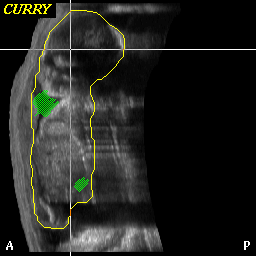
\includegraphics[width=4.339cm,height=4.339cm]{BA-img/BA-img1.png}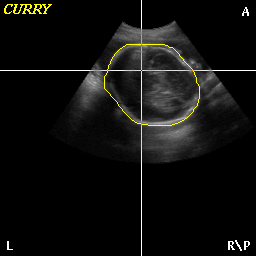
\includegraphics[width=4.339cm,height=4.339cm]{BA-img/BA-img2.png}
\captionof{figure}[Segmentierung (gelb) des Fötus in den verwendeten
Ultraschallbildern mit Pass Markers (grün).]{Segmentierung (gelb) des
Fötus in den verwendeten Ultraschallbildern mit Pass Markers (grün).}

\end{center}
\begin{center}
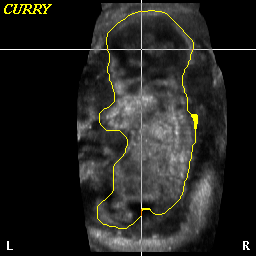
\includegraphics[width=4.339cm,height=4.339cm]{BA-img/BA-img3.png}
\end{center}
\subsubsection{Diskretisierung der Oberflächen}
Ausgehend von den Segmentierungsergebnissen wurden BEM-Modelle erstellt,
wobei die Dreiecksseitenlängen der Oberflächen in den Modellen variiert
wurden. 



\begin{center}
 [Warning: Image ignored] % Unhandled or unsupported graphics:
%\includegraphics[width=6.77cm,height=6.77cm]{graphics/fetus+vernix.tif}
 [Warning: Image ignored] % Unhandled or unsupported graphics:
%\includegraphics[width=6.77cm,height=6.77cm]{graphics/kopf+vernix.tif}
\captionof{figure}[Segmentierungsergebnisse für Fötus mit Vernix caseosa
(links) und Kopf mit Vernix caseosa (rechts) in frontaler Ansicht. Die
Vernix ist hier hautfarben dargestellt und Fötus bzw. Kopf sind
grau.]{Segmentierungsergebnisse für Fötus mit Vernix caseosa (links)
und Kopf mit Vernix caseosa (rechts) in frontaler Ansicht. Die Vernix
ist hier hautfarben dargestellt und Fötus bzw. Kopf sind grau.}
\label{seq:refIllustration1}

\end{center}
Das Segmentierungsergebnis des Fötus wurde durch Anwenden von Smoothing
und Closing mit jeweils 9mm geglättet. Durch anschließende Dilatation
um 4mm beim Fötus und 3mm beim Fötuskopf entstanden die Vernixschichten
für Fötus und Kopf (\figurename~\ref{seq:refIllustration1}). 



\begin{center}
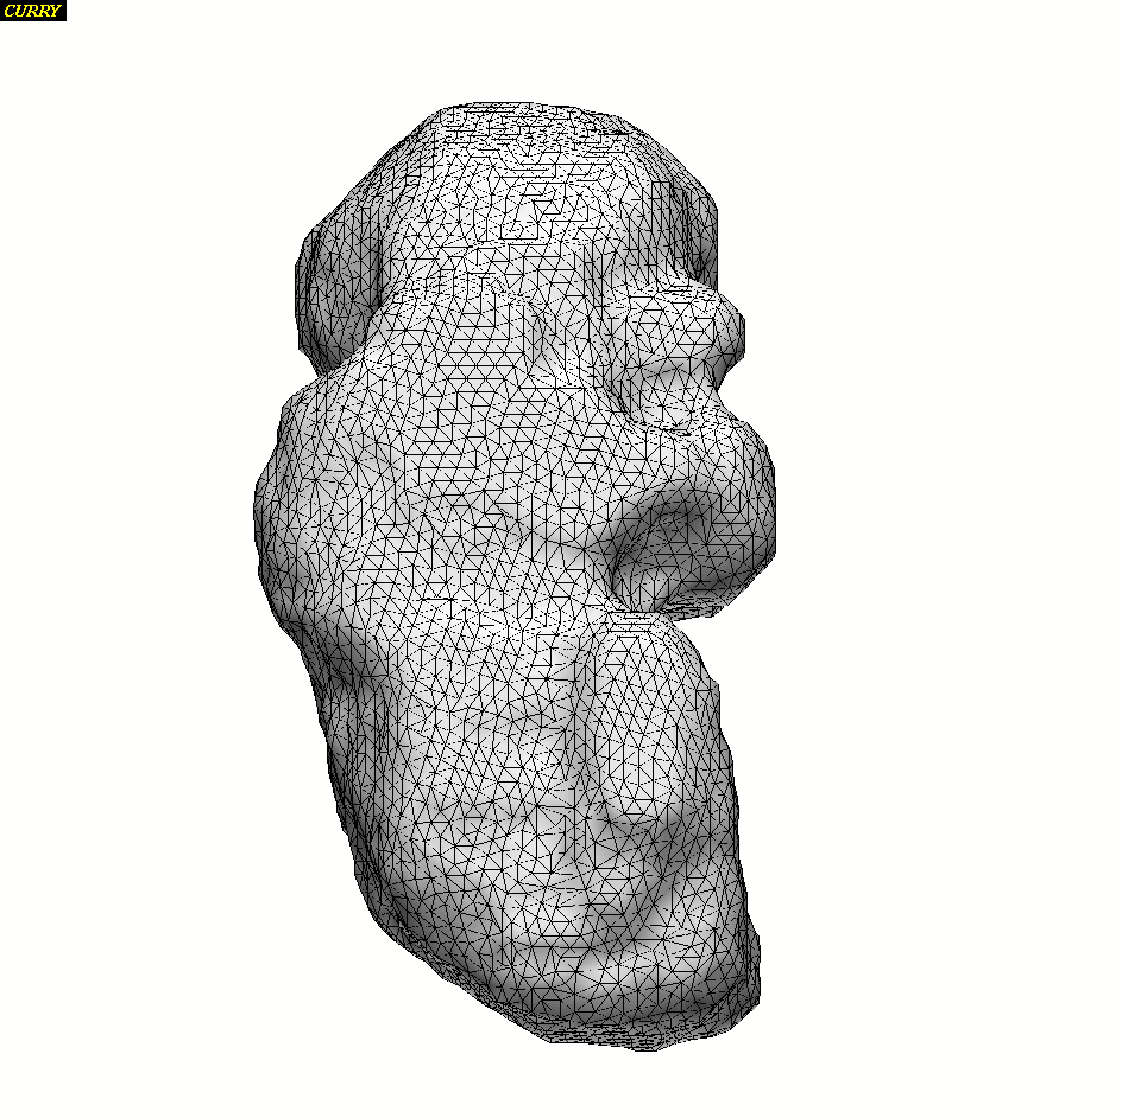
\includegraphics[width=7.92cm,height=7.99cm]{BA-img/BA-img4.pdf}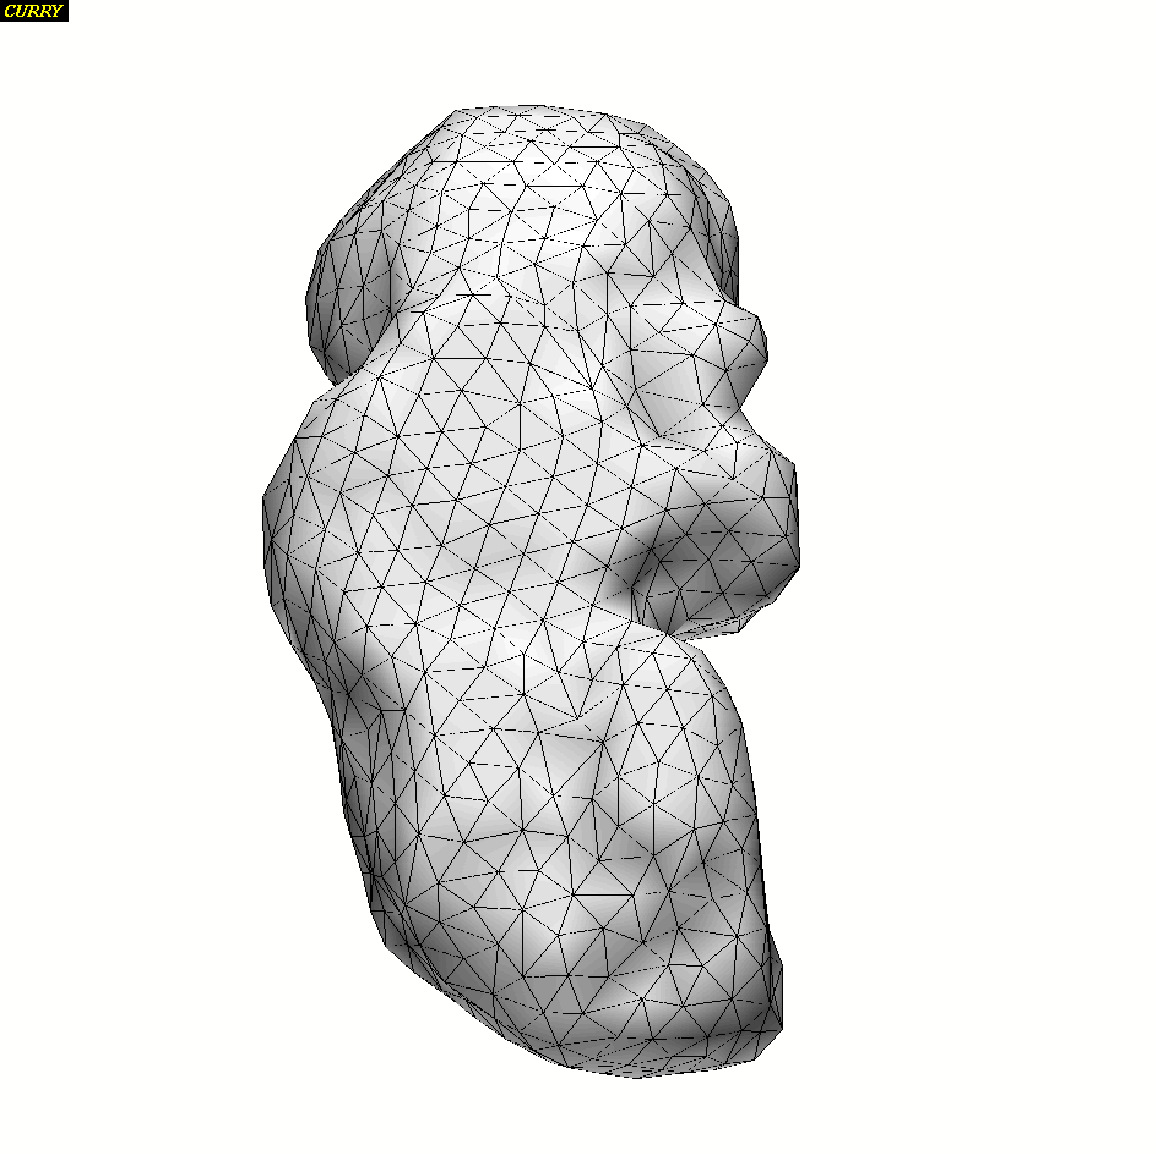
\includegraphics[width=7.92cm,height=7.99cm]{BA-img/BA-img5.pdf}
\captionof{figure}[Volumenleitermodell des Fötus mit feiner
Randelementediskretisierung (links) und grober (rechts) in frontaler
Ansicht.]{Volumenleitermodell des Fötus mit feiner
Randelementediskretisierung (links) und grober (rechts) in frontaler
Ansicht.}
\label{seq:refIllustration2}

\end{center}
Über die Oberflächen der Segmentierungen wurden Dreiecksnetze bestehend
aus Dreiecken mit definierter Dreiecksseitenlänge gelegt. Jedes dieser
Dreiecke wurde wiederum in 4 planare Unterdreiecke verfeinert um in
diesen Unterdreiecken ein stückweise konstantes Dreieckspotential
verwenden zu können.

Jedes BEM-Modell, welches in dieser Arbeit erstellt wurde, besteht aus 3
Schichten, der Fötusoberfläche, der Vernixoberfläche und der
Abdomenoberfläche. Das Abdomen ist in den BEM-Modellen die Schicht mit
den wenigsten Unebenheiten und mit der größten Oberfläche, deshalb
wurde eine größere Dreiecksseitenlängen beim Abdomen als bei den 2
inneren Schichten verwendet. Für die Vernix- und die Fötusoberfläche
wurde jeweils die gleiche Dreiecksseitenlänge gewählt, da diese sich
nur wenig unterscheiden. Das gleiche galt auch für die Kopfmodelle. Die
Dreiecksseitenlänge des Referenzmodells wurde für die inneren Schichten
mit 3mm und für das Abdomen mit 12mm festgelegt. Die Variation der
Dreiecksseitenlänge erfolgte bei den inneren Schichten in
2-mm-Schritten und beim Abdomen in 4-mm-Schritten.

\subsubsection{Modellierung und Sensorsystem}
Aus den Dreiecksnetzen von Abdomen
(\figurename~\ref{seq:refIllustration3}), Vernix caseosa und Fötus
(\figurename~\ref{seq:refIllustration2}) wurde jeweils ein 3-Schalen
BEM-Modell erstellt, sodass insgesamt 10 verschiedene, in
\tablename~\ref{seq:refTable0} aufgelistete, BEM-Modelle enstanden.



\begin{center}
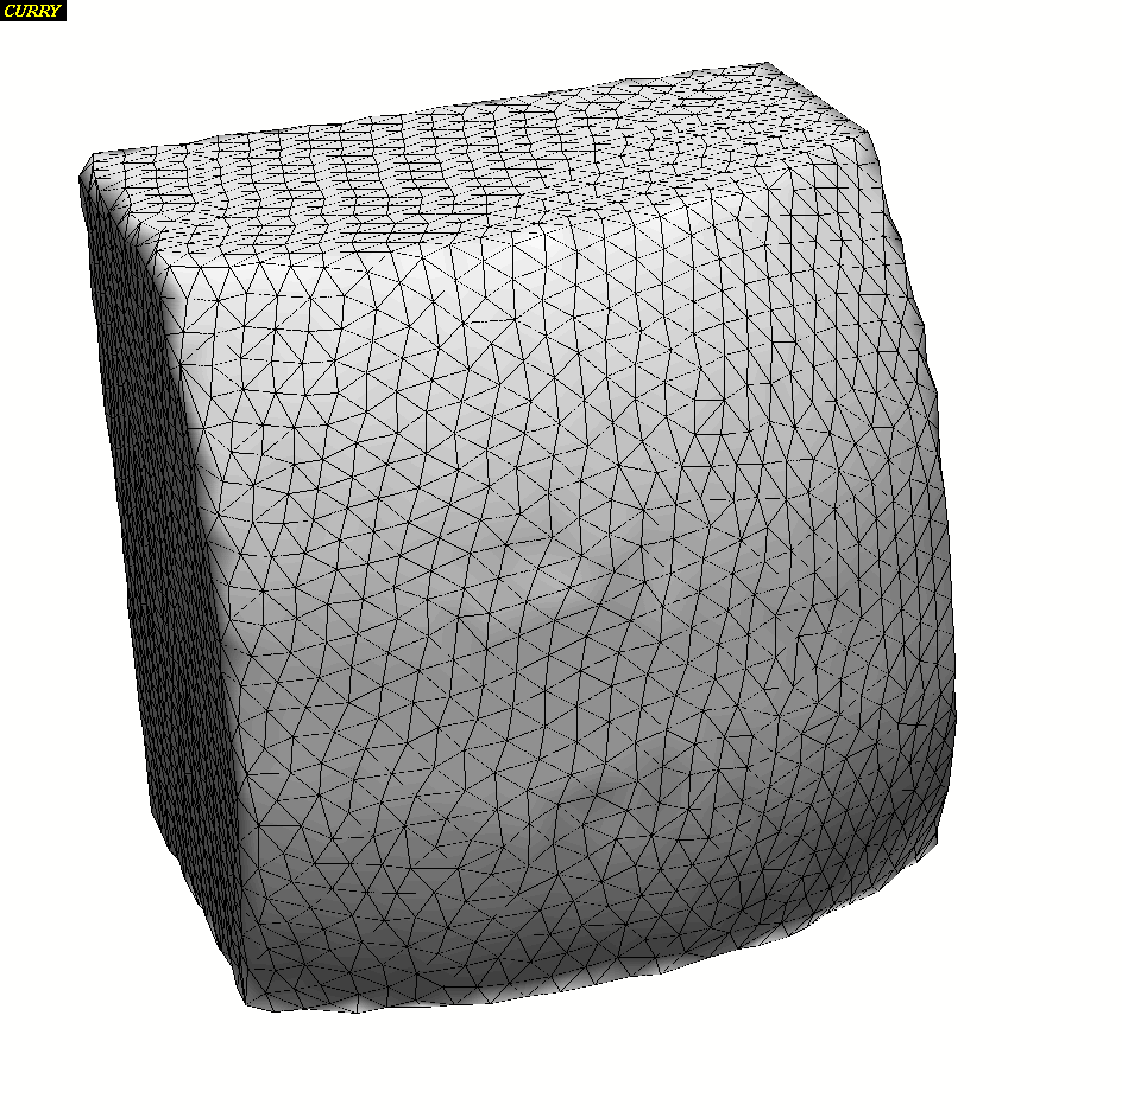
\includegraphics[width=7.92cm,height=7.99cm]{BA-img/BA-img6.pdf}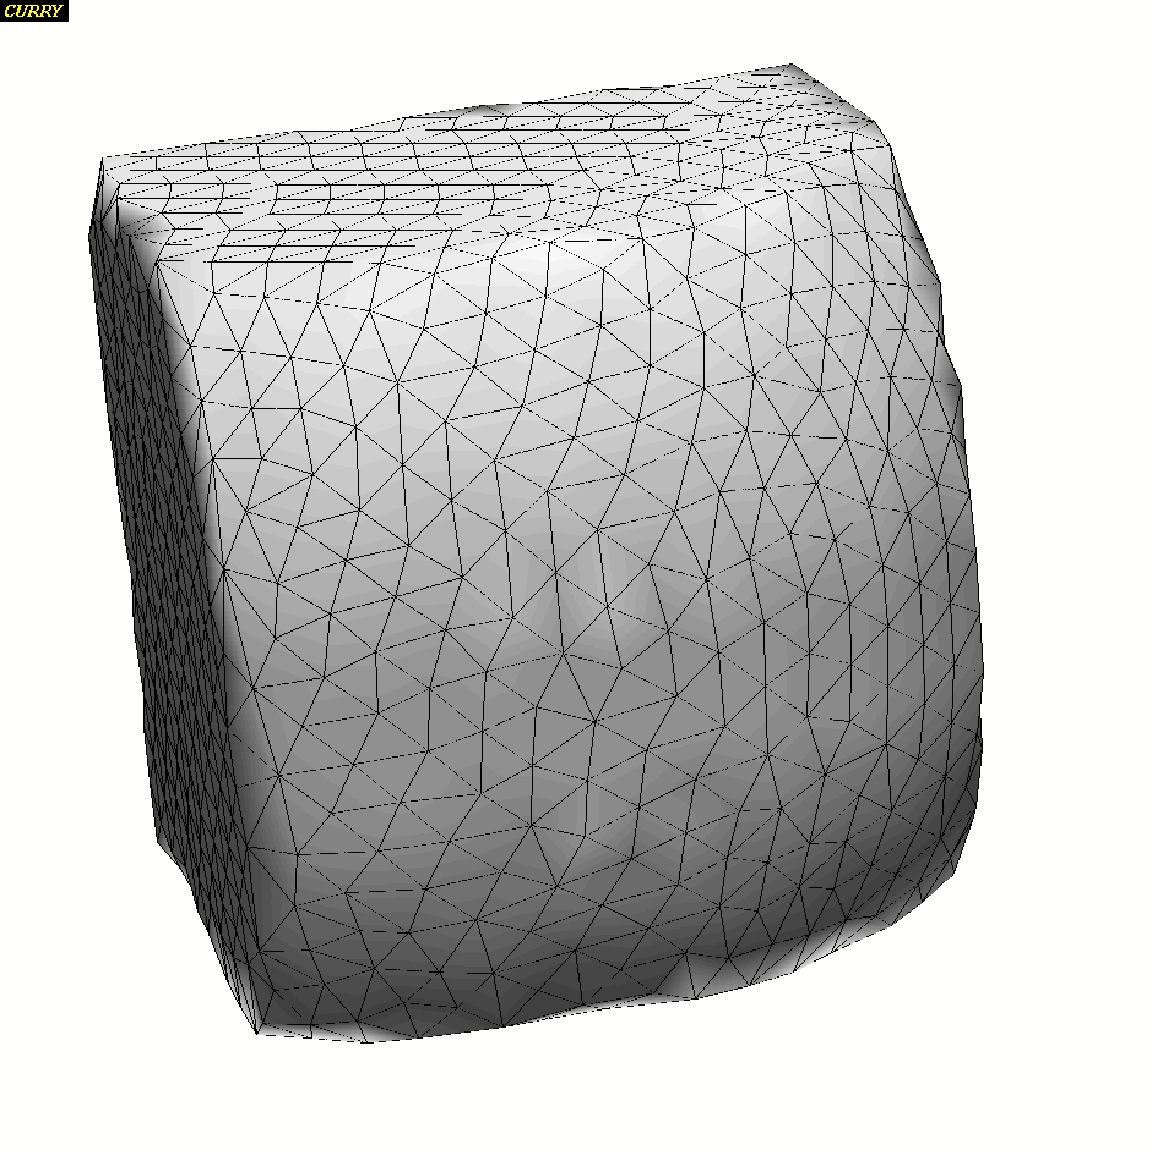
\includegraphics[width=7.99cm,height=7.99cm]{BA-img/BA-img7.pdf}
\captionof{figure}[Volumenleitermodell des Abdomens mit feinser
Randelementediskretisierung (links) und grober
(rechts).]{Volumenleitermodell des Abdomens mit feinser
Randelementediskretisierung (links) und grober (rechts).}
\label{seq:refIllustration3}

\end{center}
Um den Einfluss der Vernixschichtdicke zu überprüfen wurden noch Modelle
mit einer Vernixschichtdicke von 3mm und 2mm erstellt. Eine
Vernixschichtdicke von 2 bis 3mm enspricht den Ergebnissen von [3] und
wird hier nur mit den kleinsten Seitenlängen verwendet, da gröbere
Auflösungen bei dünnen Schichten Überschneidungen der Oberflächen
erzeugen und da nur die Auswirkungen einer Veränderung der
Vernixschichtdicke beim Fötusreferenzmodell (BEM-Modell 1 in
\tablename~\ref{seq:refTable0}) untersucht werden sollten.

\tablename~\ref{seq:refTable0} zeigt die Kombinationen der Seitenlängen
in den verschiedenen Modellen analog zu \cite{a1}:



\begin{center}
\begin{minipage}{17cm}
\captionof{table}{Übersicht über die Dreiecksseitenlängen in den
einzelnen Modellen.}
\label{seq:refTable0}
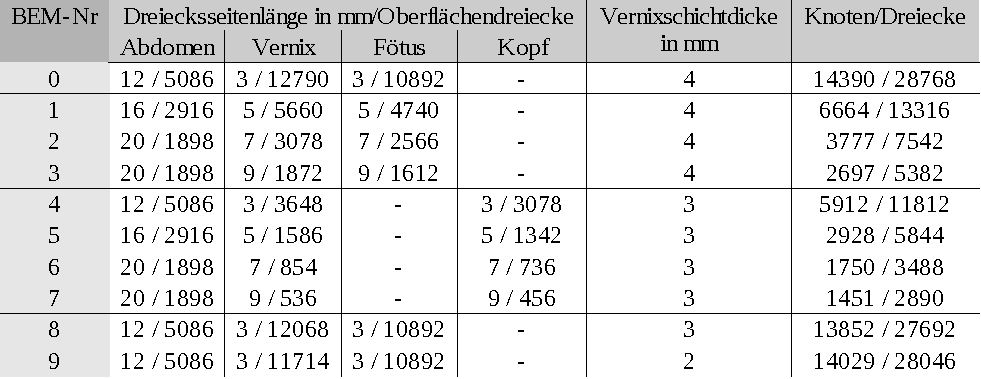
\includegraphics[width=16.018cm,height=6.412cm]{BA-img/BA-img8.pdf}\end{minipage}
\end{center}
Für das Innere jeder entstandenen Schicht wurde eine entsprechende
spezifische elektrische Leitfähigkeit definiert, dabei wurden
Leitfähigkeitswerte analog zu Werten aus \cite{a3} gewählt. In allen
BEM-Modellen wurde für das Abdomen und den Fötus bzw. den Kopf eine
spezifische elektrische Leitfähigkeit von $\sigma _{M}=\sigma
_{C}=2\cdot 10^{-1}\frac{S}{m}$ und für die Vernix eine spezifische
elektrische Leitfähigkeit von $\sigma _{V}=2\cdot 10^{-6}\frac{S}{m}$
verwendet.

Für die Simulationen und Quellenrekonstruktionen wurde das Argos-200
Sensorsystem verwendet, es hat eine feste Sensoranordnung, bestehend
aus einem hexagonalen Gitter, mit 65 Sensoren in jeder der 3
Raumesrichtungen. Die Sensoren sind in 4 planen Ebenen über dem
Messobjekt angeordnet, wobei die Ebene mit dem geringsten Abstand zum
Objekt die meisten Sensoren und die oberste Ebene nur 1 für jede der 3
unabhängigen Feldkomponenten besitzt. Die 3 oberen Sensorebenen dienen
ausschließlich der Schätzung der restlichen Rauschleistung in den
gemessenen MEG-Kanälen und wurden in dieser Arbeit in den
Vorwärtssimulationen einbezogen, aber nicht für die Lösung des inversen
Problems verwendet.



\begin{center}
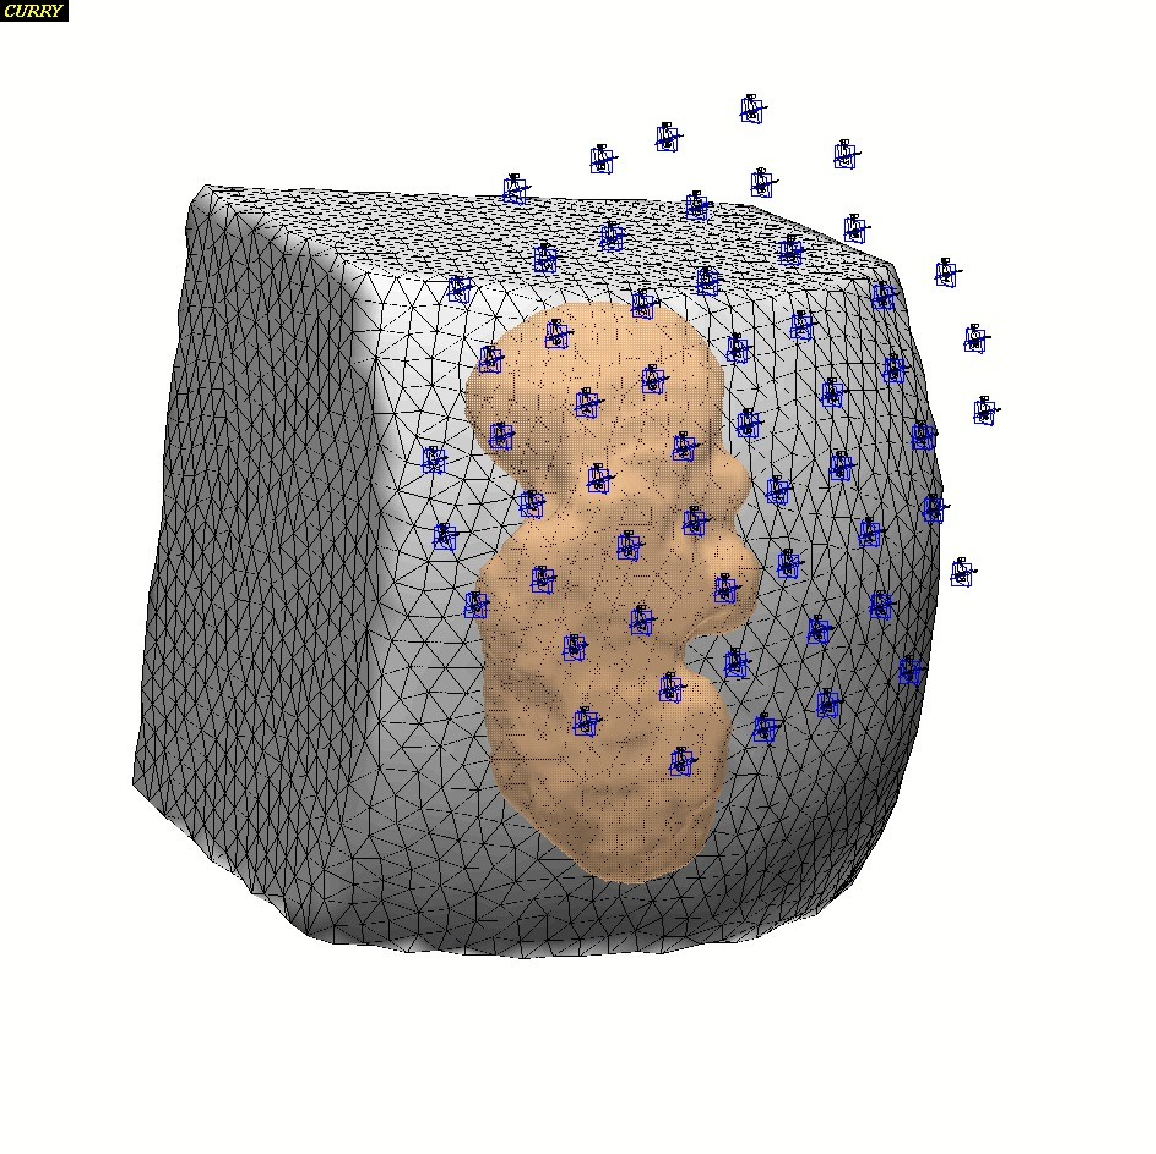
\includegraphics[width=8.721cm,height=8.784cm]{BA-img/BA-img9.pdf}
\captionof{figure}[BEM{}-Modell ausgehend von der Segmentierung des
Fötus (hautfarben) mit virtuellem SQUID{}-Sensorsystem
(blau).]{BEM-Modell ausgehend von der Segmentierung des Fötus
(hautfarben) mit virtuellem SQUID-Sensorsystem (blau).}

\end{center}
\subsection{Quellenmodell}
\subsubsection{Art der Quellen}
Als Quellen wurden bei Vorwärtsberechnungen der resultierenden Felder,
elektrische Dipole an festen Positionen mit fester Richtung definiert.
Zu verschiedenen Zeitpunkten wurden verschiedene Dipolpositionen
festgelegt, sodass bei der Vorwärtsberechnung für jeden Zeitpunkt das
Feld eines statischen Dipols berechnet wurde. Für die
Quellenrekonstruktionen wurde ein bewegter Dipol angenommen, da sich
die Position des Dipols mit der Zeit änderte. 

\subsubsection{Volume Points}
Um die Güte der Modelle für Quellen im gesamten Gehirnvolumen des Fötus
vergleichen zu können, wurde ein feines Gitter für Quellenpositionen in
dieses Volumen definiert. Um die minimale Distanz der halben
Dreiecksseitenlänge von Dipol zum nächsten Dreieck sicherzustellen,
wurde die Kopfoberfläche um 5mm erodiert. In das eingeschlossenes
Volumen wurden 1025 Quellen mit einem Abstand von 5mm verteilt. Die
Quellen wurden so verteilt, dass jede Quelle auf der Oberfläche des
eingeschlossenen Volumens einen Abstand von 5mm zu den benachbarten
Quellen hat, so entstanden 495 Oberflächenquellen, die durch die
vorangegangene Erosion einen Abstand von 5mm zur Kopfoberfläche haben.
Die inneren Quellen wurden analog zu den Oberflächenquellen erzeugt,
wobei die Oberfläche bei jedem Schritt wiederum um 6mm erodiert wurde,
bis zu dem Punkt, an dem keine Erosion mehr möglich war, dadurch
entstanden 530 innere Quellen. Insgesamt wurden 6 Quellenschichten im
Kopfvolumen erzeugt, deren Abstand radial jeweils 6mm beträgt und auf
deren Oberfläche Quellen mit einem Abstand von 5mm verteilt sind.



\begin{center}
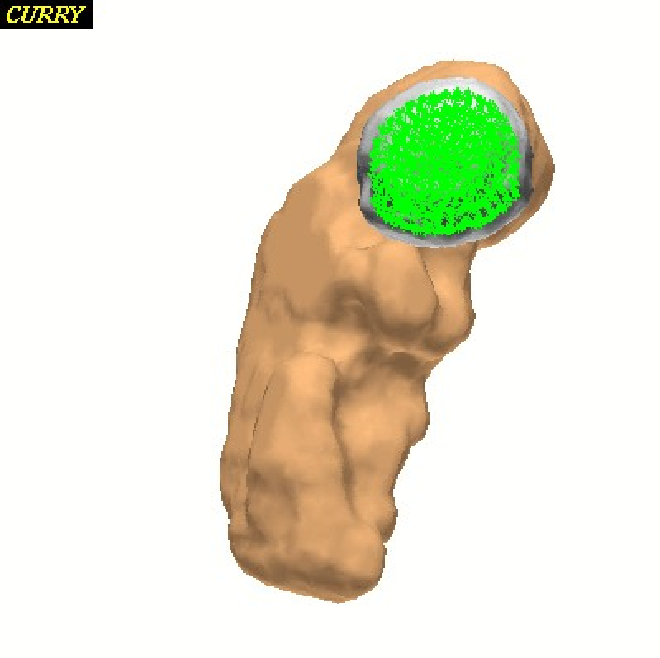
\includegraphics[width=11.19cm,height=11.16cm]{BA-img/BA-img10.pdf}
\captionof{figure}[Volumenpunkte (hellgrün) im Volumenleitermodell des
Fötus (hautfarben) und Kopfes (grau).]{Volumenpunkte (hellgrün) im
Volumenleitermodell des Fötus (hautfarben) und Kopfes (grau).}

\end{center}
\subsection{Simulation von MEG-Messdaten}
Die MEG-Feldvektoren wurden für die definierten Dipolpositionen mit 3
orthogonalen Dipolorientierungen durchgeführt an jeder Sensorposition
simuliert. Die Orientierungen der Dipole waren dabei cranial (nach
oben, zum Schädel), sinistral (nach links) und dorsal (nach hinten, zum
Rücken). Die simulierten Messdaten sind die Lösung des Vorwärtsproblems
für gegebene Quellenparameter, welches für die magnetische Flussdichte
$\boldsubformula{B}(\boldsubformula{r},\boldsubformula{r}_{Q})$ an der
Sensorposition $\boldsubformula{r}$, ausgehend von der Quellenposition
$\boldsubformula{r}_{Q}$ als

\begin{center}
\tablehead{\begin{equation*}
\begin{gathered}\boldsubformula{B}(\boldsubformula{r},\boldsubformula{r}_{Q})=-\mu
_{0}\iiint \boldsubformula{J}_{s}(\boldsubformula{r}_{Q})\times \nabla
g(\boldsubformula{r},\boldsubformula{r}_{Q})\mathit{dV}_{Q}\\+\mu
_{0}\sum _{p=1}^{n}\left[\sigma _{p}^{\text{+}}-\sigma
_{p}^{\text{{}-}}\right]\iint _{S_{p}}\Phi
(\boldsubformula{r}_{Q})\nabla
g(\boldsubformula{r},\boldsubformula{r}_{Q})\times
\boldsubformula{{\tilde {n}}}\mathit{dS}_{Q}\end{gathered}
\end{equation*}
 &
\raggedleft\arraybslash (\stepcounter{Text}{\theText})\\}
\begin{supertabular}{m{14.909cm}m{1.689cm}}

\end{supertabular}
\end{center}
definiert ist \cite{a3}. In dieser Gleichung ist $S_{p}$ die Oberfläche,
welche zwei Schichten der Leitfähigkeiten $\sigma _{p}^{\text{+}}$ und
$\sigma _{p}^{\text{{}-}}$ voneinander trennt. Der nach Außen
gerichtete Normalenvektor der Oberfläche $S_{p}$ wurde mit
$\boldsubformula{{\tilde {n}}}$ bezeichnet. Für das biologische Gewebe
wurde die magnetische Permittivität $\mu _{0}$ des Vakuums angenommen. 
$\boldsubformula{J}_{S}(\boldsubformula{r}_{Q})$ ist die Stromdichte
und $\Phi (\boldsubformula{r}_{Q})$ ist das Potential an der
Dipolposition $\boldsubformula{r}_{Q}$ . Für homogene, isotrope
Kompartimente lässt sich die Greensche Funktion als
$g(\boldsubformula{r},\boldsubformula{r}_{Q})=\frac{\mu _{0}}{4\pi
\|\boldsubformula{r}-\boldsubformula{r}_{Q}\|}$ formulieren.



\begin{center}
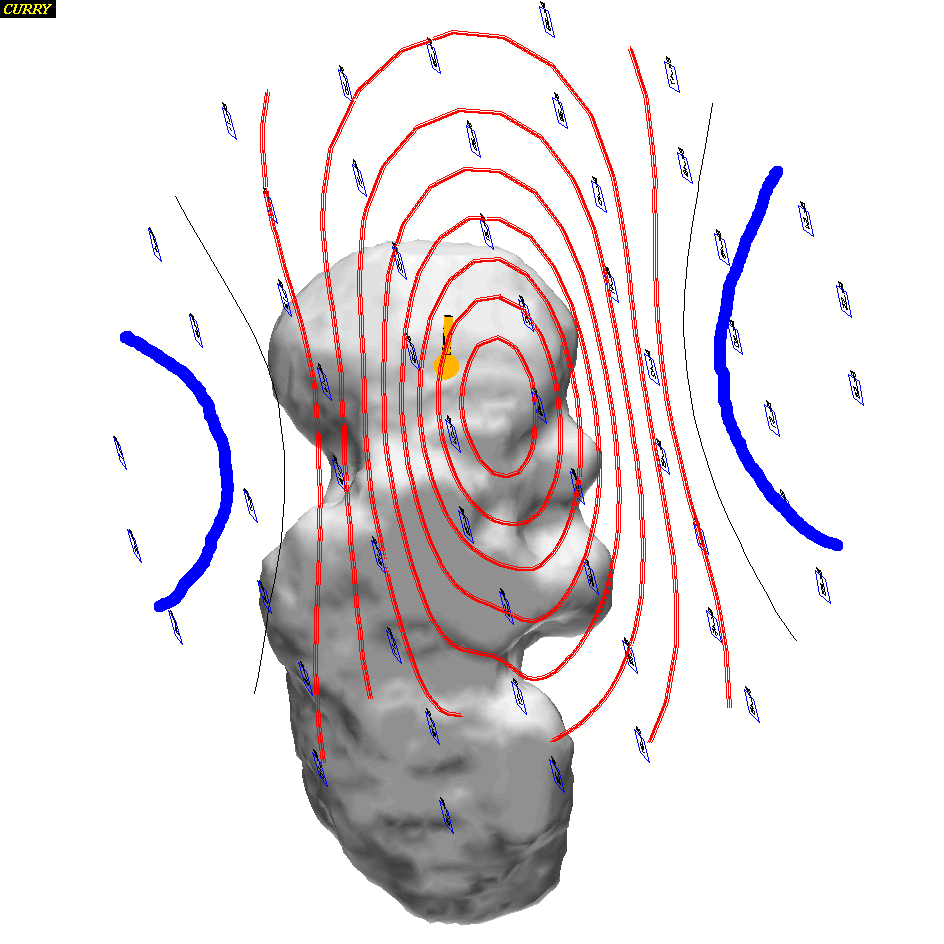
\includegraphics[width=4.791cm,height=4.791cm]{BA-img/BA-img11.png}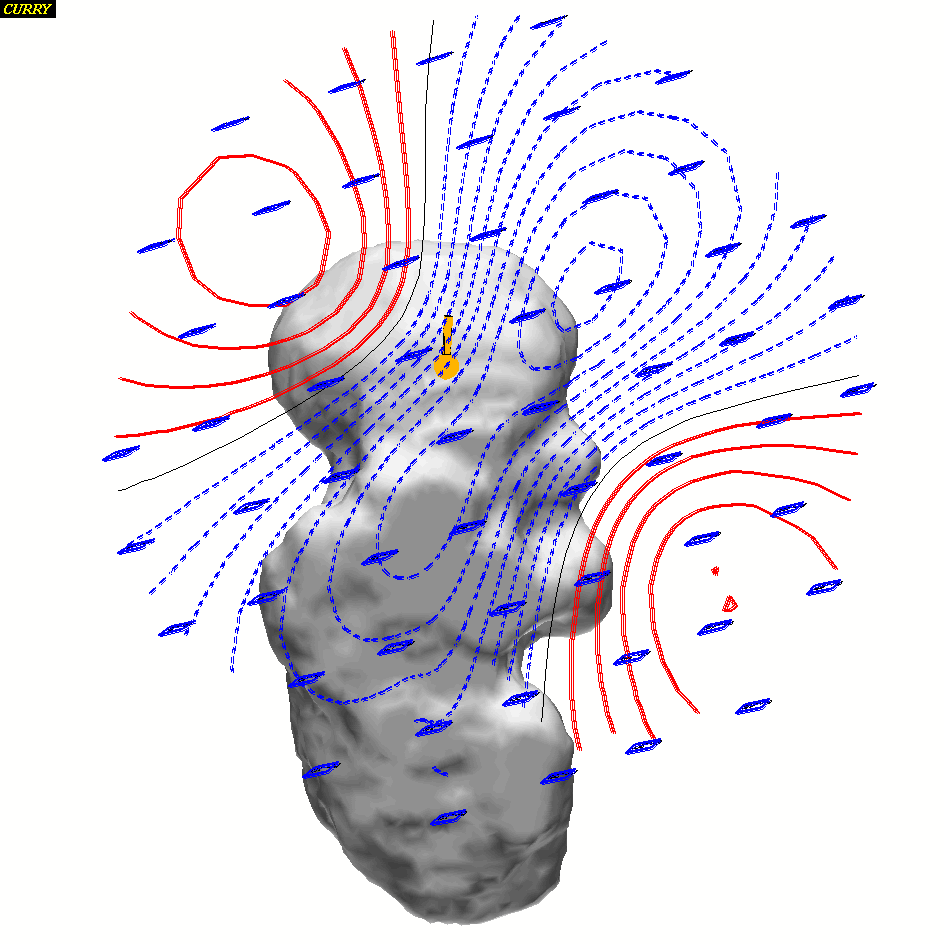
\includegraphics[width=4.791cm,height=4.791cm]{BA-img/BA-img12.png}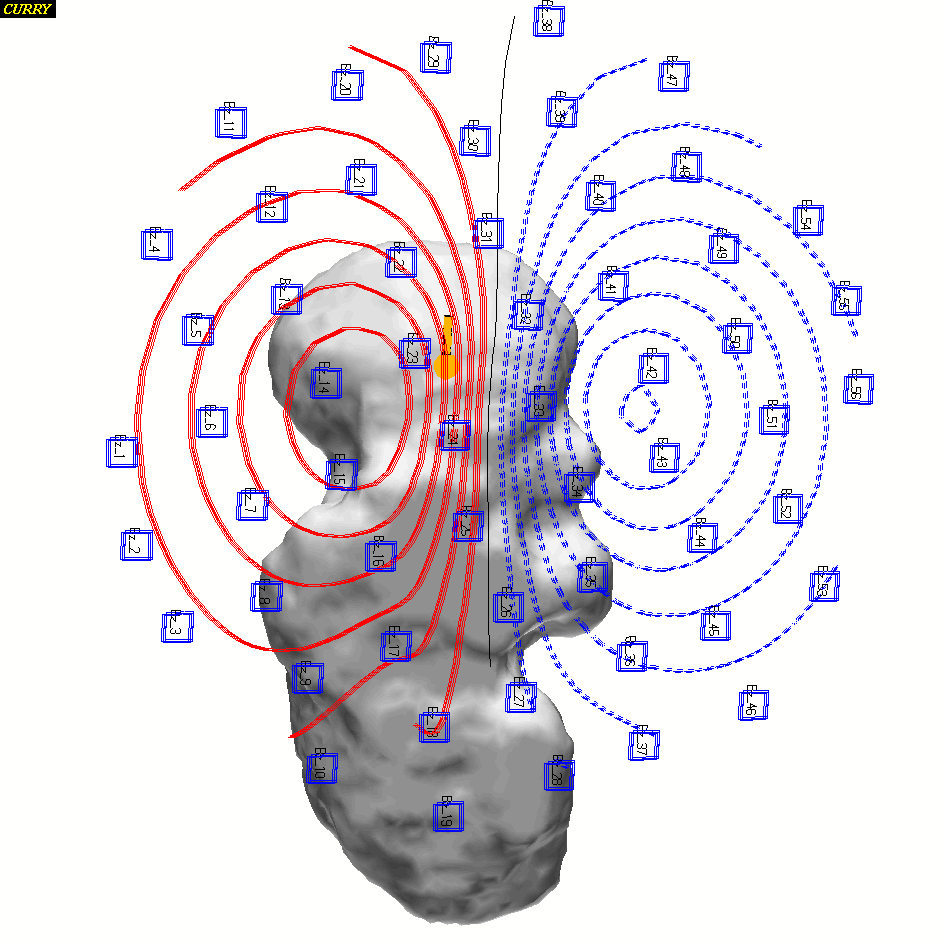
\includegraphics[width=4.791cm,height=4.791cm]{BA-img/BA-img13.png}
\captionof{figure}[Feldbilder einer Simulation mit cranialer
Dipolorientierung im Fötusmodell in den drei Sensorausrichtungen x
(links), y (mitte) und z (rechts) in frontaler Ansicht.]{Feldbilder
einer Simulation mit cranialer Dipolorientierung im Fötusmodell in den
drei Sensorausrichtungen x (links), y (mitte) und z (rechts) in
frontaler Ansicht.}

\end{center}
In den Simulationen wurde für jeden Zeitpunkt ein anderer Dipolort
verwendet, sodass eine Zeitreihe mit 1025 verschiedenen Feldbildern
entstand. Für die Vorwärtsrechnung wurden stückweise konstante
Dreieckspotentiale in den Unterdreiecken verwendet.

\subsection{Rekonstruktion simulierter Messdaten}
Mit den simulierten Messwerten für die Felder des Referenzmodells
BEM-Modell 0, wurden für jedes Modell Quellenrekonstruktionen
durchgeführt. Dabei wurden als a priori Information die Dipolpositionen
vorgegeben. Die Rekonstruktion beschränkte sich also auf
Dipolorientierung und Dipolstärke. Quellenrekonstruktionen wurden mit
jedem Model für alle drei Dipolorientierungen (cranial, dorsal und
sinistral) durchgeführt. Bei der Lösung des inversen Problems wurden
wie bei der Vorwärtsrechnung stückweise konstante Potentiale der
Unterdreiecke verwendet und es wurde als isoliertes Problem betrachtet
ohne quasisphärische Korrekturen. Bei Quasisphärischer Korrektur werden
ausschließlich tangential gerichtete Dipole benutzt, da das MEG ca. 6-
bis 10mal sensitiver gegenüber tangentialen Dipolen verglichen mit
radialen Dipolen ist \cite{a2}, was die Berechnungen für annähernd
sphärische Volumenleiter verbessert [?CURRY REFERENCE MANUAL].

Die Lösung des inversen Problems verwendet die Gleichung

\begin{center}
\tablehead{\begin{equation*}
\boldsubformula{B}=\boldsubformula{L}\boldsubformula{J}+n
\end{equation*}
 &
\raggedleft\arraybslash (\stepcounter{Text}{\theText})\\}
\begin{supertabular}{m{14.909cm}m{1.689cm}}

\end{supertabular}
\end{center}
und stellte diese nach J um. Dabei ist $\boldsubformula{L}$ die
Lead-field Matrix und \textit{n} ist die Rauschkomponente, welche in
diesem Spezialfall der simulierten Messdaten wegfällt.

\subsection{Bewertung von Simulation und Rekonstruktion}
\subsubsection{Simulationsbewertung}
Von den Simulierten Feldern wurden jeweils die \textit{relative
difference measures}/RDM und Amplitudenfaktoren/MAG zu den jeweiligen
Referenzfeldern berechnet. Die Referenzfelder für die Fötusmodelle
stammten von dem Fötusmodell mit den kleinsten Dreiecksseitenlängen.
Die Felder der Kopfmodelle wurden mit den Referenzfeldern des
Fötusmodells und mit den Feldern des höchstaufgelösten Kopfmodells
verglichen.

Die erste Kennzahl zur Bewertung der Simulationsergebnisse ist der
\textit{relative difference measure }(\textit{RDM}) der analog zu
\cite{a5} definiert ist als

\begin{center}
\tablehead{\centering  $\mathit{RDM}=\sqrt{\sum
_{i=1}^{n}\left(\frac{\mathit{meas}_{i}}{\sum
_{j=1}^{n}{\mathit{meas}_{j}^{2}}}-\frac{\mathit{ref}_{i}}{\sum
_{j=1}^{n}{\mathit{ref}_{j}^{2}}}\right)^{2}}$, &
\raggedleft\arraybslash (\stepcounter{Text}{\theText})\\}
\begin{supertabular}{m{14.909cm}m{1.689cm}}

\end{supertabular}
\end{center}
wobei $n$ die Anzahl der Sensoren ist und $\mathit{ref}_{i}$ und
$\mathit{meas}_{i}$ die \textit{i}ten Komponenten des simulierten
Feldvektors für das jeweilige Referenzmodell und das abweichende Modell
sind. Der \textit{RDM} ist eine Größe für den topographischen Fehler
(minimaler Fehler: $\mathit{RDM}=0$). Die zweite Differenzgröße ist der
Amplitudenfaktor (\textit{MAG}), wie in \cite{a5} definiert als

\begin{center}
\tablehead{\centering  $\mathit{MAG}=\sqrt{\frac{\sum
_{i=1}^{n}{\mathit{meas}_{i}^{2}}}{\sum
_{i=1}^{n}{\mathit{ref}_{i}^{2}}}}$, &
\raggedleft\arraybslash (\stepcounter{Text}{\theText})\\}
\begin{supertabular}{m{14.909cm}m{1.689cm}}

\end{supertabular}
\end{center}
somit ist der Amplitudenfaktor \textit{MAG} ein Maß für den Fehler der
Amplituden (minimaler Fehler: $\mathit{MAG}=1$).

Die Aufteilung des Fehlers der berechneten Felder in \textit{RDM} und
\textit{MAG} ist daher sinnvoll, da eine Änderung der Amplitude
(\textit{MAG}) die rekonstruierte Dipolstärke beeinflusst aber nicht
die räumliche Lokalisierung, eine Topologieänderung wirkt sich hingegen
immer auf die räumliche Lokalisierung aus \cite{a2}. Von den gesuchten
Größen (\textit{RDM} und \textit{MAG}) wurden jeweils der Mittelwert
und die Standardabweichung über alle Zeitschritte und somit über alle
Quellenpositionen ermittelt.

\subsubsection{Rekonstruktionsbewertung}
Bei der Quellenrekonstruktion wurden die verwendeten Dipolpositionen
vorgegeben und damit nur die Orientierungen und Amplituden der Dipole
rekonstruiert. Die Bewertung der Orientierungen in den
Rekonstruktionsergebnissen erfolgt über den Winkel $\alpha $ zwischen
den Richtungsvektoren des jeweiligen Simulationsdipols $\vec{s}$ und
des dazugehörigen rekonstruierten Dipols $\vec{r}$ mit dem Zusammenhang

\begin{center}
\tablehead{\centering  $\alpha =\arccos \left(\frac{\vec{r}\cdot
\vec{s}}{\left|{\vec{r}}\right|\cdot \left|{\vec{s}}\right|}\right)$. &
\raggedleft\arraybslash (\stepcounter{Text}{\theText})\\}
\begin{supertabular}{m{14.909cm}m{1.689cm}}

\end{supertabular}
\end{center}
Der Winkel $\alpha $ ist damit ein Maß für den Fehler der
rekonstruierten Dipolrichtung (minimaler Fehler: $\alpha =0$). Der
Amplitudenfaktor für den rekonstruierten Dipol ist der Quotient $a$ aus
den Beträgen des rekonstruierten Dipols und des entsprechenden
Simulationsdipols

\begin{center}
\tablehead{\begin{equation*}
a=\frac{\left|{\vec{r}}\right|}{\left|{\vec{s}}\right|}
\end{equation*}
 &
\raggedleft\arraybslash (\stepcounter{Text}{\theText})\\}
\begin{supertabular}{m{14.909cm}m{1.689cm}}

\end{supertabular}
\end{center}
und gibt den Fehler der rekonstruierten Dipolstärke an (minimaler
Fehler: $a=1$).

Diese Kennzahlen wurden für jeden der 1025 Dipole berechnet.

\subsubsection{Statistische Auswertung}
Die Bewertungsgrößen (\textit{RDM}, \textit{MAG},  $\alpha $  und
\textit{a}) werden für jeden Dipolort bestimmt und sind damit
vektorielle Größen. 

RDM und MAG-Ergebnisse liegen für alle drei Sensorausrichtungen (x, y
und z) vor, um deren Verteilungen mit Mittelwert und Standardabweichung
zu beschreiben, müssen Mittelwert  $\mu $ von Mittelwerten

\begin{center}
\tablehead{\begin{equation*}
\mu =E[\left(\frac{1}{N}\sum _{i=1}^{N}X_{i}\right)]
\end{equation*}
 &
\raggedleft\arraybslash (\stepcounter{Text}{\theText})\\}
\begin{supertabular}{m{14.909cm}m{1.689cm}}

\end{supertabular}
\end{center}
und Varianz  $\sigma ^{2}$  von Mittelwerten berechnet werden

\begin{center}
\tablehead{\centering  $\sigma ^{2}=V[\left(\frac{1}{N}\sum
_{i=1}^{N}X_{i}\right)]=\frac{1}{N^{2}}\left(\sum _{i=1}^{N}\sum
_{j=1}^{N}\mathit{cov}[X_{i},X_{j}]\right)$ . &
\raggedleft\arraybslash (\stepcounter{Text}{\theText})\\}
\begin{supertabular}{m{14.909cm}m{1.689cm}}

\end{supertabular}
\end{center}
